\documentclass[a4paper,twoside,openright]{article}
%\documentclass[a4paper,oneside,openright]{book}

% Prepare for svenska tecken
\usepackage[T1]{fontenc}
\usepackage[swedish]{babel}
%\usepackage[]{geometry}
\addto\captionsswedish{\renewcommand{\figurename}{Bild}}
\usepackage{amsmath}
\usepackage{fancyhdr}
\usepackage{wrapfig}
\usepackage{caption}
\usepackage{framed}
\usepackage[fulladjust]{marginnote}
\usepackage{color}
\newcommand{\hilight}[1]{\colorbox{yellow}{#1}}
\usepackage{hyperref}
\hypersetup{
    colorlinks,
    citecolor=black,
    filecolor=black,
    linkcolor=black,
    urlcolor=black
}
\usepackage{stmaryrd} % För symbolen \boxbox, kräver paketet texlive-math-extra

% % % % % % % % % % % 
% Detta är nya environments för review. De bör vara relativt självförklarande hur de används.
% I princip sätter man bara den del av texten som har en viss status mellan\begin{rev-granskat} och \end{rev-granskat} tex.
% Undvik att nästla dem för det är ingen idé det fungerar inte.
% De är testade med ett antal andra environemnt som tabular mm men kolla att det fungerar med de environments du använder.
% % % % % % % % % % % % % % % % % % % % % % % % % % % % % % % % % % % % % % % % % % % % % % % % % % % % % % % % % % % % % % % 
\usepackage[svgnames,rgb]{xcolor}
\usepackage{pdfcomment}
\newenvironment{rev-ogranskat}{\begin{pdfsidelinecomment}[color=black,linewidth=3px,caption=inline]{Ogranskat}}{\end{pdfsidelinecomment}}
\newenvironment{rev-omarbetas}{\begin{pdfsidelinecomment}[color=red,linewidth=3px,caption=inline]{Omarbetas}}{\end{pdfsidelinecomment}}
\newenvironment{rev-raderas}{\begin{pdfsidelinecomment}[color=red,linewidth=3px,caption=inline]{Raderas}}{\end{pdfsidelinecomment}}
\newenvironment{rev-redo}{\begin{pdfsidelinecomment}[color=yellow,linewidth=3px,caption=inline]{Redo att granska}}{\end{pdfsidelinecomment}}
\newenvironment{rev-granskat}[1][]%
{\begin{pdfsidelinecomment}[color=green,linewidth=3px,caption=inline]%
{Granskat #1}}%
{\end{pdfsidelinecomment}}
\newenvironment{rev-nytt}[1][]%
{\begin{pdfsidelinecomment}[color=brown,linewidth=3px,caption=inline]%
{Nytt #1}}%
{\end{pdfsidelinecomment}}
\newenvironment{rev-releasat}{\begin{pdfsidelinecomment}[color=blue,linewidth=3px,caption=inline]{Klart}}{\end{pdfsidelinecomment}}

\clubpenalty=9990
\widowpenalty=9999
\brokenpenalty=4999

\usepackage[europeanvoltages,europeancurrents,europeanresistors,cuteinductors,smartlabels]{circuitikz}
\usepackage[framemethod=TikZ]{mdframed}

\mdfdefinestyle{FactBox}{%
    linecolor=blue,
    outerlinewidth=2pt,
    roundcorner=20pt,
    innertopmargin=\baselineskip,
    innerbottommargin=\baselineskip,
    innerrightmargin=20pt,
    innerleftmargin=20pt,
    backgroundcolor=gray!50!white}
\newcommand{\infobox}[1]{
\begin{wrapfigure}{r}{0.5\textwidth}
  \begin{mdframed}[style=FactBox]
#1
  \end{mdframed}
\end{wrapfigure}
}

% Prepare for tables
\usepackage{multirow}
\usepackage{longtable}

% Prepare for lists
\usepackage{enumitem}

% Prepare for graphics
\usepackage{xspace,graphicx}

\raggedbottom

% Prepare for version handling
\usepackage{xstring}
\usepackage{catchfile}
\CatchFileDef{\HEAD}{.git/refs/heads/master}{}
\newcommand{\gitrevision}{%
  \StrLeft{\HEAD}{7}%
}
\CatchFileDef{\VERSION}{VERSION.txt}{}
\newcommand{\revision}{%
  \VERSION \gitrevision%
}

%% Frontpage bacground
\usepackage{eso-pic}
\newcommand\BackgroundPic{%
\put(0,0){%
\parbox[b][\paperheight]{\paperwidth}{%
\vfill
\centering
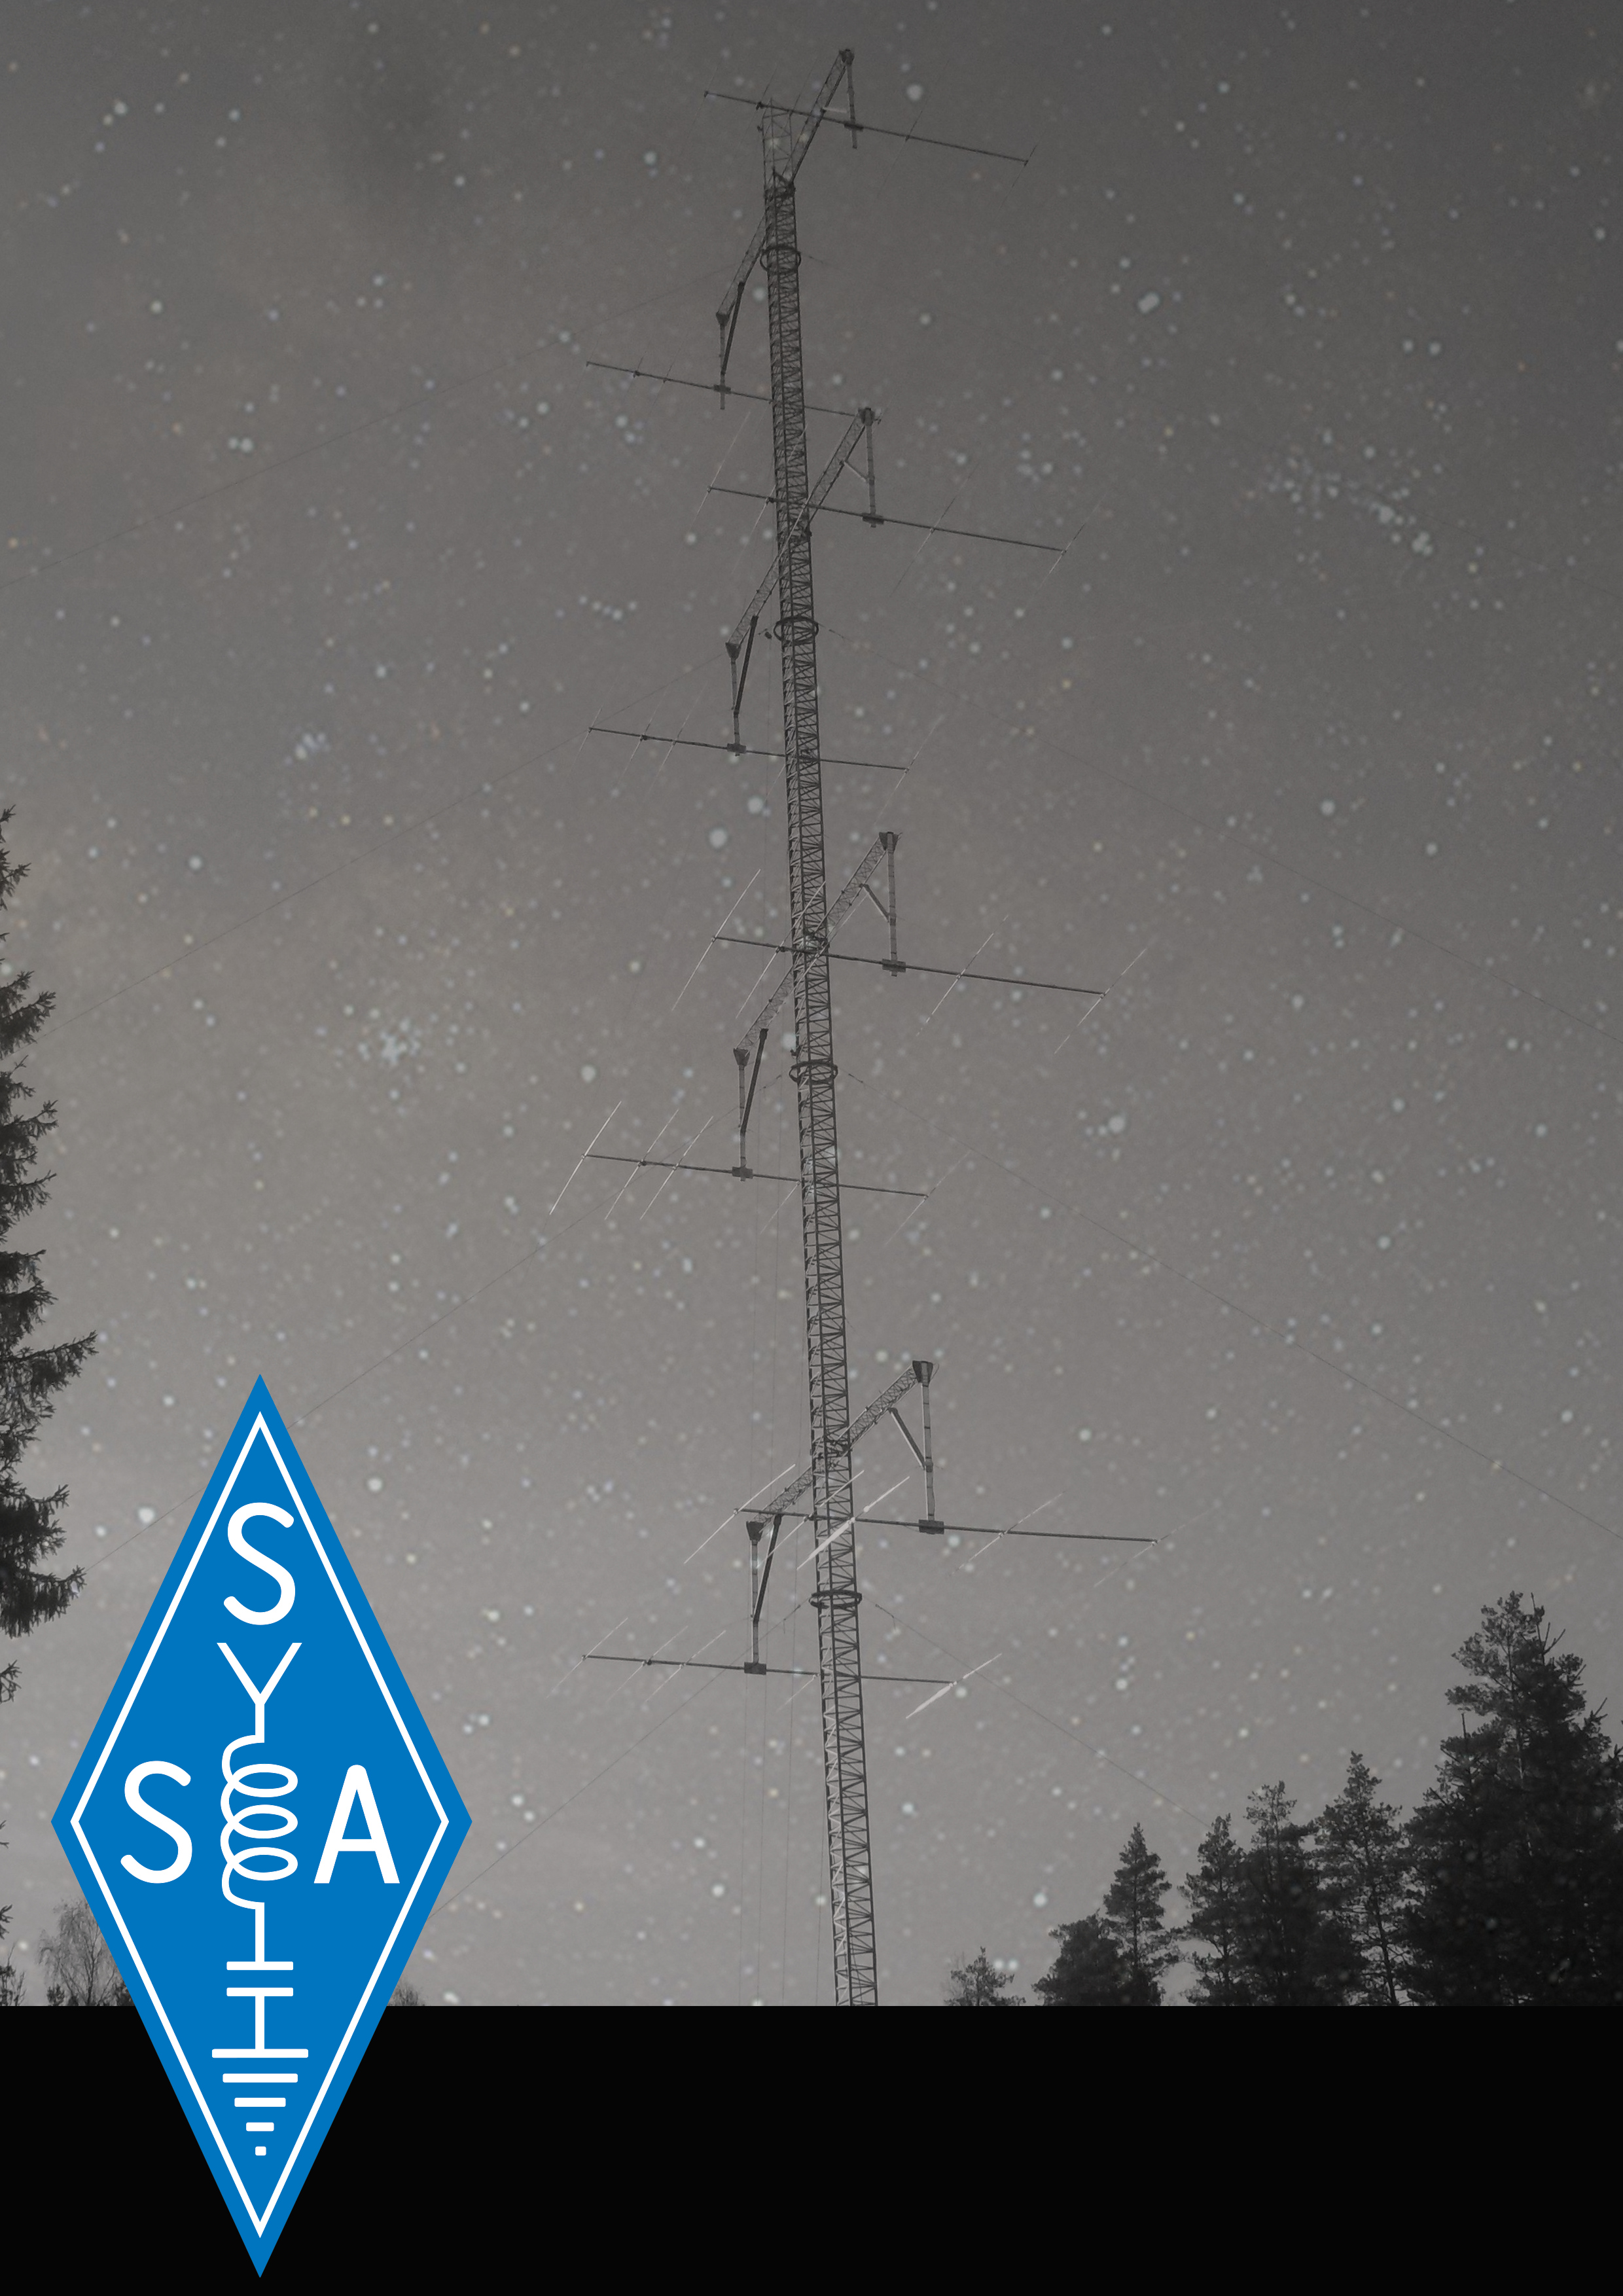
\includegraphics[width=\paperwidth,height=\paperheight,%
keepaspectratio]{images/koncept-front.jpg}%
\vfill
}}}


\newcommand\Backgroundtwo{%
\put(0,0){%
\parbox[b][\paperheight]{\paperwidth}{%
\vfill
\centering
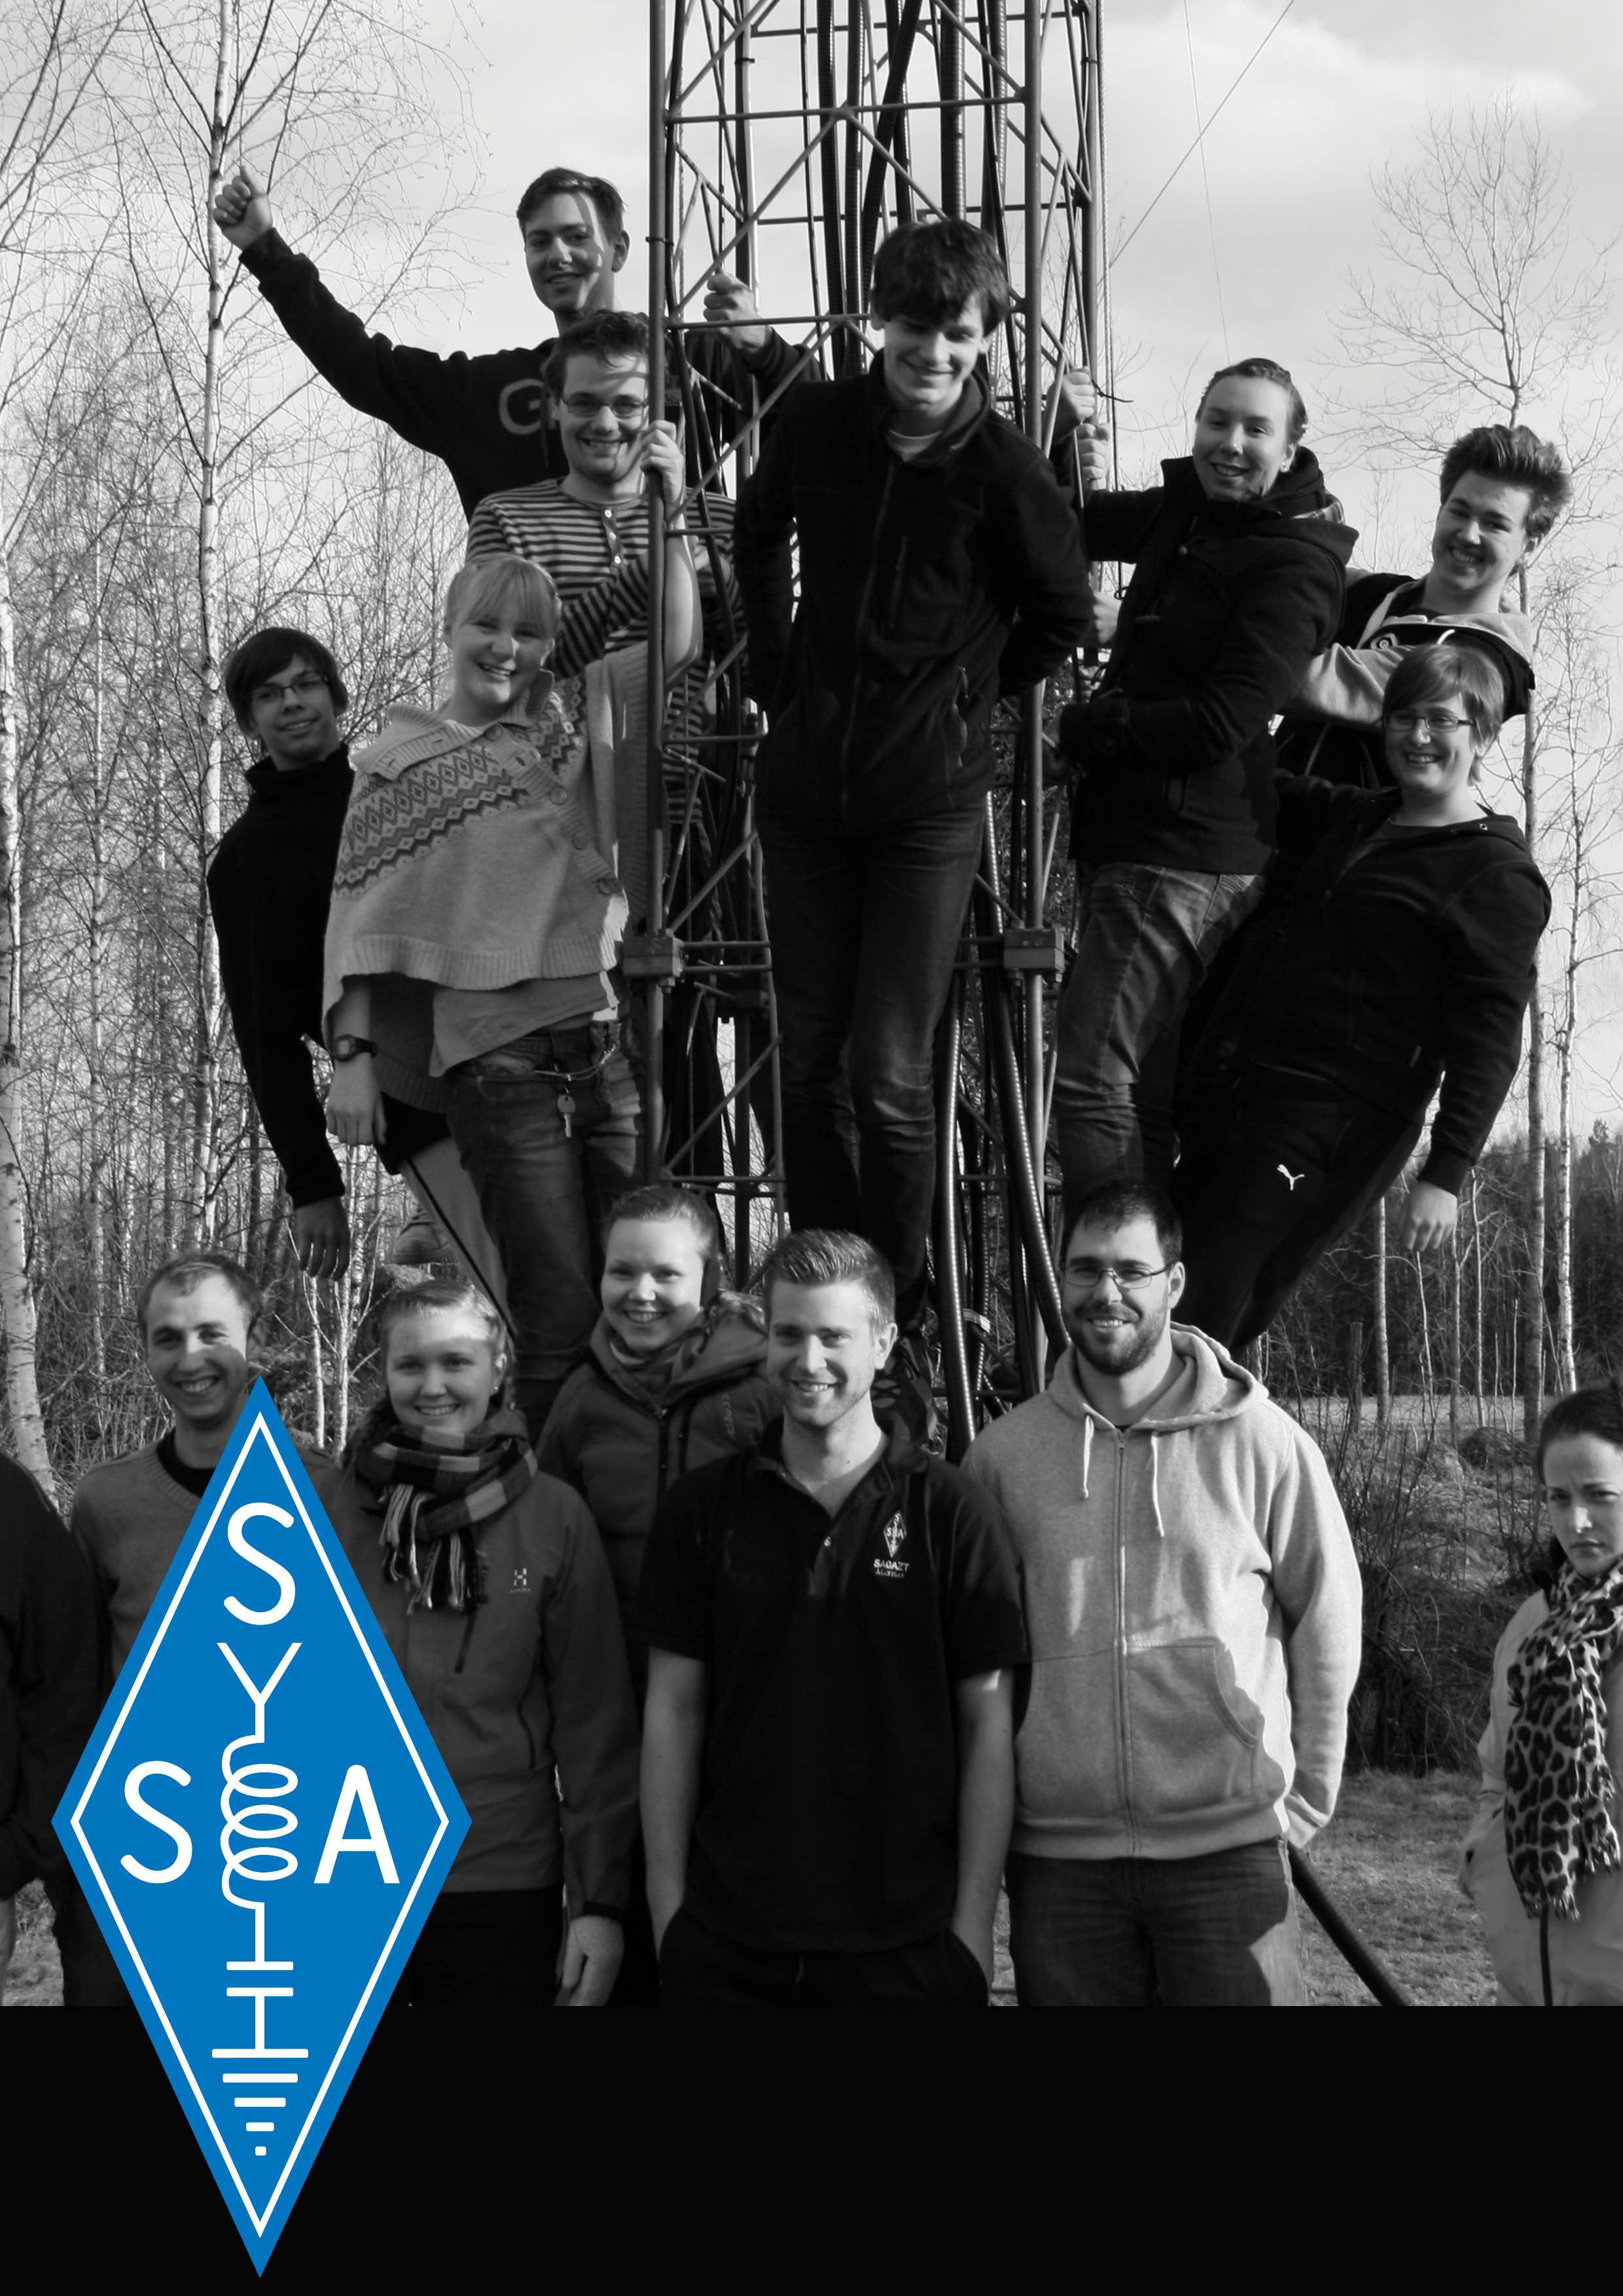
\includegraphics[width=\paperwidth,height=\paperheight,%
keepaspectratio]{images/koncept-larobok-front.jpg}%
\vfill
}}}



\newcommand\BackgroundPicLast{%
\put(0,0){%
\parbox[b][\paperheight]{\paperwidth}{%
\vfill
\centering

\includegraphics[width=\paperwidth,height=\paperheight,%
keepaspectratio]{images/koncept-back.pdf}%
\vfill
}}}

%tlfällig fix för kompilering%
\nonstopmode
\usepackage[swedish]{babel}

\headheight = 12.6pt

% Prepare for abstract
\pagestyle{plain}
\newenvironment{abstract}%
{\cleardoubblanklepage\null \vfill\begin{center}\bfseries Abstract \end{center}}%
%{\cleardoublepage\null \vfill\begin{center}%
%\bfseries \abstractname \end{center}}%
     {\vfill\null}

\usepackage{refbook}

% Prepare for index
\usepackage{makeidx}
\makeindex

\begin{document}
\frontmatter
%\mainmatter
% Frontpage

\title{Kursplan för Koncept}
\author{Magnus Danielson SA0MAD}
\maketitle

\section*{Introduktion}

Denna kursplan baseras på den kurs som Täby Sändaramatörer TSA/SK0MT håller.
Den är uppdelad i 14 lektioner.
Ellära och reglemente lektionerna ligger om varandra för att eleverna skall
hinna smälta saker och läsa ikapp.
Ett praktiskt moment är inlagt för att bygga vanor och släppa mikronfon-rädslan.
På slutet finns ett tillfälle för repetition och frågor, samt ett sista
tillfälle där ett prov gås igenom.

Läsanvisningar till boken ``Koncept för Amatörradiocertifikat, andra upplagan''
anges per lektion, jämte de däri liggande HAREC-kraven.
Som appendix finns även de detaljerade HAREC-kraven, så man som referens kan se
i vilken lektion som de hanteras.
Detta försäkrar att alla kraven kan täckas av lektioner.

\lfoot[\revision]{}
\rfoot[]{\revision}

\cleardoublepage
\pagestyle{fancy}


\tableofcontents

\setlength{\parindent}{0pt}
\setlength{\parskip}{1ex plus 0.5ex minus 0.2ex}

\mainmatter

\section{Introduktion och Ellära}

\subsection{Introduktion}

Kort introduktion om kursen, kursledare och lärare samt det praktiska.
Utdelning av böcker. Sen följer en mjukstart för att få med sig de flesta.

\subsection{Matematik}
Bilaga B.1 Uttryck
\textbf{HAREC I.\ref{HAREC.I.c.1}\label{myHAREC.I.c.1}}
\textbf{HAREC I.\ref{HAREC.I.c.2}\label{myHAREC.I.c.2}}
\textbf{HAREC I.\ref{HAREC.I.c.6}\label{myHAREC.I.c.6}}

Bilaga B.2 Formler
\textbf{HAREC I.\ref{HAREC.I.d}\label{myHAREC.I.d.2a}}

Bilaga B.3 Exempel med 1 obekant
\textbf{HAREC I.\ref{HAREC.I.d}\label{myHAREC.I.d.2b}}

Bilaga B.5 Potenser, digniteter
\textbf{HAREC I.\ref{HAREC.I.c.4}\label{myHAREC.I.c.4}}

Bilaga B.6 Rötter
\textbf{HAREC I.\ref{HAREC.I.c.5}\label{myHAREC.I.c.5}}

Bilaga B.7 Logaritmer
\textbf{HAREC I.\ref{HAREC.I.c.3}\label{myHAREC.I.c.3}}

Bilaga B.8 Binära tal
\textbf{HAREC I.\ref{HAREC.I.c.8}\label{myHAREC.I.c.8}}

\subsection{Ellära}

Kapitel 1.1.4 Konduktivitet - Ledare, halvledare och isolator
\textbf{HAREC a.\ref{HAREC.a.1.1}\label{myHAREC.a.1.1}, a.\ref{HAREC.a.1.1.1}\label{myHAREC.a.1.1.1}}

Kapitel 1.1.5 Elektrisk spänning -- Enheten volt
\textbf{HAREC a.\ref{HAREC.a.1.1.2}\label{myHAREC.a.1.1.2b}, a.\ref{HAREC.a.1.1.3}\label{myHAREC.a.1.1.3b}}

Kapitel 1.1.7 Elektrisk ström -- Enheten ampere
\textbf{HAREC a.\ref{HAREC.a.1.1.2}\label{myHAREC.a.1.1.2a}, a.\ref{HAREC.a.1.1.3}\label{myHAREC.a.1.1.3a}}

Kapitel 1.1.10 Resistans -- Enheten ohm
\textbf{HAREC a.\ref{HAREC.a.1.1.2}\label{myHAREC.a.1.1.2c}, a.\ref{HAREC.a.1.1.3}\label{myHAREC.a.1.1.3c}}

Kapitel 1.1.11 Ohms lag
\textbf{HAREC a.\ref{HAREC.a.1.1.4}\label{myHAREC.a.1.1.4}}

Kapitel 1.1.12 Kirchhoffs lagar
\textbf{HAREC a.\ref{HAREC.a.1.1.5}\label{myHAREC.a.1.1.5}}

Kapitel 1.1.13 Elektrisk effekt -- Enheten watt
\textbf{HAREC a.\ref{HAREC.a.1.1.6}\label{myHAREC.a.1.1.6}, a.\ref{HAREC.a.1.1.7}\label{myHAREC.a.1.1.7}}

Kapitel 1.1.15 Joules lag
\textbf{HAREC a.\ref{HAREC.a.1.1.8}\label{myHAREC.a.1.1.8}}

Kapitel 1.1.17 Amperetimmar (Ah) och batterikapacitet
\textbf{HAREC a.\ref{HAREC.a.1.1.9}\label{myHAREC.a.1.1.9}}

Kapitel 1.2.1 Elektromotorisk kraft -- EMK
\textbf{HAREC a.\ref{HAREC.a.1.2}\label{myHAREC.a.1.2}, a.\ref{HAREC.a.1.2.1}\label{myHAREC.a.1.2.1}} 

Kapitel 1.2.2 Serie- och parallellkopplade kraftkällor
\textbf{HAREC a.\ref{HAREC.a.1.2.2}\label{myHAREC.a.1.2.2}}

\section{Amatörradiotermer & Reglemente}

\section{Ellära - DC}
\section{Ellära - AC}

\section{Elsäkerhet}
\section{Ellära - radioteknik}
\section{Radiosändare}
\section{Radiomottagare}
\section{Praktik HF/VHF}
\section{Antenner}

\section{Vågutbredning}
\section{EMC/EMF}
\section{Repetition, frågor}
\section{Genomgång av övningsskrivning}

\appendix

\chapter{CEPT HAREC krav}

Den här upplagan av KonCEPT är baserad på CEPT T/R 61-02 Harmonised Amatuer Radio
Examination Certificate (HAREC) Edition 4 June 2016. För att underlätta att se
att alla HAREC-kraven finns täckta samt se vilka HAREC krav som en viss textdel
uppfyller.

För den studerande så kan detta hjälpa till att förstå hur omfattande kraven är
från den internationella överenskommelsen som CEPT HAREC är. Det är genom dessa
gemensamma minimumregler som jämförbarheten i kunskap länder emellan sedan kan
utföras.

Själva kunskapskraven i HAREC finns beskrivna i ''Annex 6: Examination syllabus and requirements for a HAREC''. Alla krav i den finns med här, i HAREC
orginalformulering, enbart omarbetad med avseende på format. För varje krav
redovisas sedan en eller flera referenser i den övriga texten där det kravet
anses uppfyllas.

I bokens text står det \textbf{HAREC a.\ref{HAREC.a.1.4}} där magnetfält behandlas
för att referera till HAREC-kravet 1.4 Magnetic field;. Samma ställe refereras
sedan från kravet med del-kapitel inom paratens (\ref{myHAREC.a.1.4}).

\section{Introduction}

\makeatletter
\renewcommand{\theenumii}{\arabic{enumii}}
\renewcommand{\labelenumii}{\theenumi.\theenumii}
\renewcommand{\p@enumii}{\theenumi.}

\renewcommand{\theenumiii}{\arabic{enumiii}}
\renewcommand{\labelenumiii}{\theenumi.\theenumii.\theenumiii}
\renewcommand{\p@enumiii}{\theenumi.\theenumii.}
\makeatother

\begin{enumerate}[label=\alph*.]
\item Where quantities are referred to, candidates should know the units in which these quantities are expressed, as well as the generally used multiples and sub-multiples of these units. (\ref{myHAREC.I.a})\label{HAREC.I.a}
\item Candidates must be familiar with the compound of the symbols. (\ref{myHAREC.I.b})\label{HAREC.I.b}
\item Candidates must know the following mathematical concepts and operations:
\begin{enumerate}
\item adding, subtracting, multiplying and dividing (\ref{myHAREC.I.c.1})\label{HAREC.I.c.1}
\item fractions (\ref{myHAREC.I.c.2})\label{HAREC.I.c.2}
\item powers of ten, exponentials, logarithms (\ref{myHAREC.I.c.3})\label{HAREC.I.c.3}
\item squaring (\ref{myHAREC.I.c.4})\label{HAREC.I.c.4}
\item square roots (\ref{myHAREC.I.c.5})\label{HAREC.I.c.5}
\item inverse values (\ref{myHAREC.I.c.6})\label{HAREC.I.c.6}
\item interpretation of linear and non-linear graphs (\ref{myHAREC.I.c.7})\label{HAREC.I.c.7}
\item binary number system (\ref{myHAREC.I.c.8})\label{HAREC.I.c.8}
\end{enumerate}
\item Candidates must be familiar with the formulae used in this syllabus and be able to transpose them. (\ref{myHAREC.I.d})\label{HAREC.I.d}
\end{enumerate}

\section{Technical Content}

\makeatletter
\renewcommand{\labelenumi}{\theenumi.}

\renewcommand{\theenumii}{\arabic{enumii}}
\renewcommand{\labelenumii}{\theenumi.\theenumii}
\renewcommand{\p@enumii}{\theenumi.}

\renewcommand{\theenumiii}{\arabic{enumiii}}
\renewcommand{\labelenumiii}{\theenumi.\theenumii.\theenumiii}
\renewcommand{\p@enumiii}{\theenumi.\theenumii.}

\renewcommand{\theenumiv}{\arabic{enumiv}}
\renewcommand{\labelenumiv}{\theenumi.\theenumii.\theenumiii.\theenumiv}
\renewcommand{\p@enumiv}{\theenumi.\theenumii.\theenumiii.}
\makeatother

\begin{enumerate}
\item ELECTRICAL, ELECTRO-MAGNETIC AND RADIO THEORY
\begin{enumerate}

\item Conductivity; (\ref{myHAREC.a.1.1})\label{HAREC.a.1.1}
\begin{enumerate}
\item Conductor, semiconductor and insulator; (\ref{myHAREC.a.1.1.1})\label{HAREC.a.1.1.1}
\item Current (\ref{myHAREC.a.1.1.2a}), voltage (\ref{myHAREC.a.1.1.2b}) and resistance; (\ref{myHAREC.a.1.1.2c})\label{HAREC.a.1.1.2}
\item The units ampere (\ref{myHAREC.a.1.1.3a}), volt (\ref{myHAREC.a.1.1.3b}) and ohm; (\ref{myHAREC.a.1.1.3c})\label{HAREC.a.1.1.3}
\item Ohm's Law  \(\left[E = I \cdot R\right]\); (\ref{myHAREC.a.1.1.4})\label{HAREC.a.1.1.4}
\item Kirchhoff's Laws; (\ref{myHAREC.a.1.1.5})\label{HAREC.a.1.1.5}
\item Electric power \(\left[P = E \cdot I\right]\); (\ref{myHAREC.a.1.1.6})\label{HAREC.a.1.1.6}
\item The unit watt; (\ref{myHAREC.a.1.1.7})\label{HAREC.a.1.1.7}
\item Electric energy \(\left[W = P \cdot t\right]\); (\ref{myHAREC.a.1.1.8})\label{HAREC.a.1.1.8}
\item The capacity of a battery [ampere-hour]. (\ref{myHAREC.a.1.1.9})\label{HAREC.a.1.1.9}
\end{enumerate}

\item Sources of electricity; (\ref{myHAREC.a.1.2})\label{HAREC.a.1.2}
\begin{enumerate}
\item Voltage source, source voltage [EMF], short circuit current, inter­nal resistance and terminal voltage; (\ref{myHAREC.a.1.2.1})\label{HAREC.a.1.2.1}
\item Series and parallel connection of voltage sources. (\ref{myHAREC.a.1.2.2})\label{HAREC.a.1.2.2}
\end{enumerate}

\item Electric field; (\ref{myHAREC.a.1.3})\label{HAREC.a.1.3}
\begin{enumerate}
\item Electric field strength; (\ref{myHAREC.a.1.3.1})\label{HAREC.a.1.3.1}
\item The unit volt/meter; (\ref{myHAREC.a.1.3.2})\label{HAREC.a.1.3.2}
\item Shielding of electric fields. (\ref{myHAREC.a.1.3.3})\label{HAREC.a.1.3.3}
\end{enumerate}

\item Magnetic field; (\ref{myHAREC.a.1.4})\label{HAREC.a.1.4}
\begin{enumerate}
\item Magnetic field surrounding live conductor; (\ref{myHAREC.a.1.4.1})\label{HAREC.a.1.4.1}
\item Shielding of magnetic fields. (\ref{myHAREC.a.1.4.2})\label{HAREC.a.1.4.2}
\end{enumerate}

\item Electromagnetic field; (\ref{myHAREC.a.1.5})\label{HAREC.a.1.5}
\begin{enumerate}
\item Radio waves as electromagnetic waves; (\ref{myHAREC.a.1.5.1})\label{HAREC.a.1.5.1}
\item Propagation velocity and its relation with frequency and wavelength \(\left[v = \lambda \cdot f\right]\); (\ref{myHAREC.a.1.5.2})\label{HAREC.a.1.5.2}
\item Polarisation. (\ref{myHAREC.a.1.5.3})\label{HAREC.a.1.5.3}
\end{enumerate}

\item Sinusoidal signals; (\ref{myHAREC.a.1.6})\label{HAREC.a.1.6}
\begin{enumerate}
\item The graphic representation in time; (\ref{myHAREC.a.1.6.1})\label{HAREC.a.1.6.1}
\item Instantaneous value (\ref{myHAREC.a.1.6.2a})\label{HAREC.a.1.6.2a}, amplitude [Emax] (\ref{myHAREC.a.1.6.2b})\label{HAREC.a.1.6.2b}, effective [RMS] value (\ref{myHAREC.a.1.6.2c})\label{HAREC.a.1.6.2c} and average value \(\left[U_{eff} = \frac{U_{max}}{\sqrt{2}}\right]\) (\ref{myHAREC.a.1.6.2d})\label{HAREC.a.1.6.2d};
\item Period (\ref{myHAREC.a.1.6.3a})\label{HAREC.a.1.6.3a} and duration of period (\ref{myHAREC.a.1.6.3b})\label{HAREC.a.1.6.3b};
\item Frequency; (\ref{myHAREC.a.1.6.4})\label{HAREC.a.1.6.4}
\item The unit hertz; (\ref{myHAREC.a.1.6.5})\label{HAREC.a.1.6.5}
\item Phase difference. (\ref{myHAREC.a.1.6.6})\label{HAREC.a.1.6.6}
\end{enumerate}

\item Non-sinusoidal signals, noise; (\ref{myHAREC.a.1.7})\label{HAREC.a.1.7}
\begin{enumerate}
\item Audio signals; (\ref{myHAREC.a.1.7.1})\label{HAREC.a.1.7.1}
\item Square wave; (\ref{myHAREC.a.1.7.2})\label{HAREC.a.1.7.2}
\item The graphic representation in time; (\ref{myHAREC.a.1.7.3})\label{HAREC.a.1.7.3}
\item D.C. voltage component (\ref{myHAREC.a.1.7.4a})\label{HAREC.a.1.7.4a}, fundamental wave and higher harmonics (\ref{myHAREC.a.1.7.4b})\label{HAREC.a.1.7.4b};
\item Noise \(\left[P_N=TB\right]\)(receiver thermal noise, band noise, noise density, noise power in receiver bandwidth).  (\ref{myHAREC.a.1.7.5})\label{HAREC.a.1.7.5}
\end{enumerate}

\item Modulated signals; (\ref{myHAREC.a.1.8})\label{HAREC.a.1.8}
\begin{enumerate}
\item CW; (\ref{myHAREC.a.1.8.1})\label{HAREC.a.1.8.1}
\item Amplitude modulation; (\ref{myHAREC.a.1.8.2})\label{HAREC.a.1.8.2}
\item Phase modulation (\ref{myHAREC.a.1.8.3a})\label{HAREC.a.1.8.3a}, frequency modulation (\ref{myHAREC.a.1.8.3b})\label{HAREC.a.1.8.3b} and single-sideband modulation (\ref{myHAREC.a.1.8.3c})\label{HAREC.a.1.8.3c};
\item Frequency deviation and modulation index \(\left[m = \frac{\Delta F}{f_{mod}}\right]\); (\ref{myHAREC.a.1.8.4})\label{HAREC.a.1.8.4}
\item Carrier, sidebands and bandwidth; (\ref{myHAREC.a.1.8.5})\label{HAREC.a.1.8.5}
\item Waveforms of CW (\ref{myHAREC.a.1.8.6a})\label{HAREC.a.1.8.6a}, AM (\ref{myHAREC.a.1.8.6b})\label{HAREC.a.1.8.6b}, SSB (\ref{myHAREC.a.1.8.6c})\label{HAREC.a.1.8.6c} and FM (\ref{myHAREC.a.1.8.6d})\label{HAREC.a.1.8.6d} signals (graphical presentation);
\item Spectrum of CW (\ref{myHAREC.a.1.8.7a})\label{HAREC.a.1.8.7a}, AM (\ref{myHAREC.a.1.8.7b})\label{HAREC.a.1.8.7b} and SSB (\ref{myHAREC.a.1.8.7c})\label{HAREC.a.1.8.7c} signals (graphical presentation);
\item Digital modulations (\ref{myHAREC.a.1.8.8})\label{HAREC.a.1.8.8}: FSK (\ref{myHAREC.a.1.8.8a})\label{HAREC.a.1.8.8a}, 2-PSK (\ref{myHAREC.a.1.8.8b})\label{HAREC.a.1.8.8b}, 4-PSK (\ref{myHAREC.a.1.8.8c})\label{HAREC.a.1.8.8c}, QAM (\ref{myHAREC.a.1.8.8d})\label{HAREC.a.1.8.8d};
\item Digital modulation (\ref{myHAREC.a.1.8.9})\label{HAREC.a.1.8.9}: bit rate (\ref{myHAREC.a.1.8.9a})\label{HAREC.a.1.8.9a}, symbol rate (Baud rate) (\ref{myHAREC.a.1.8.9b})\label{HAREC.a.1.8.9b} and bandwidth (\ref{myHAREC.a.1.8.9c})\label{HAREC.a.1.8.9c};
\item CRC (\ref{myHAREC.a.1.8.10a})\label{HAREC.a.1.8.10a} and retransmissions (e.g. packet radio) (\ref{myHAREC.a.1.8.10b})\label{HAREC.a.1.8.10b}, forward error correction (e.g. Amtor FEC) (\ref{myHAREC.a.1.8.10c})\label{HAREC.a.1.8.10c}.
\end{enumerate}

\item Power and energy; (\ref{myHAREC.a.1.9})\label{HAREC.a.1.9}
\begin{enumerate}
\item The power of sinusoidal signals \(\left[P=i^2 \cdot R; P=\frac{u^2}{R}; u=U_{eff}; i=I_{eff}\right]\); (\ref{myHAREC.a.1.9.1})\label{HAREC.a.1.9.1}
\item Power ratios corresponding to the following dB values: 0 dB, 3 dB, 6 dB, 10 dB and 20 dB [both positive and negative]; (\ref{myHAREC.a.1.9.2})\label{HAREC.a.1.9.2}
\item The input/output power ratio in dB of series-connected amplifiers and/or attenuators; (\ref{myHAREC.a.1.9.3})\label{HAREC.a.1.9.3}
\item Matching [maximum power transfer]; (\ref{myHAREC.a.1.9.4})\label{HAREC.a.1.9.4}
\item The relation between power input and output and efficiency \(\left[\eta=\frac{P_{out}}{P_{in}}\cdot 100\%\right]\); (\ref{myHAREC.a.1.9.5})\label{HAREC.a.1.9.5}
\item Peak Envelope Power [p.e.p.]. (\ref{myHAREC.a.1.9.6})\label{HAREC.a.1.9.6}
\end{enumerate}

\item Digital signal processing (DSP).
\begin{enumerate}
\item sampling and quantization; (\ref{myHAREC.a.1.10.1})\label{HAREC.a.1.10.1}
\item minimum sampling rate (Nyquist frequency); (\ref{myHAREC.a.1.10.2})\label{HAREC.a.1.10.2}
\item convolution (time domain / frequency domain, graphical presentation); (\ref{myHAREC.a.1.10.3})\label{HAREC.a.1.10.3}
\item anti-aliasing filtering, reconstruction filtering; (\ref{myHAREC.a.1.10.4})\label{HAREC.a.1.10.4}
\item ADC / DAC. (\ref{myHAREC.a.1.10.5})\label{HAREC.a.1.10.5}
\end{enumerate}

\end{enumerate}

\item COMPONENTS
\begin{enumerate}
\item Resistor; (\ref{myHAREC.a.2.1})\label{HAREC.a.2.1}
\begin{enumerate}
\item The unit ohm; (\ref{myHAREC.a.2.1.1})\label{HAREC.a.2.1.1}
\item Resistance; (\ref{myHAREC.a.2.1.2})\label{HAREC.a.2.1.2}
\item Current/voltage characteristic; (\ref{myHAREC.a.2.1.3})\label{HAREC.a.2.1.3}
\item Power dissipation. (\ref{myHAREC.a.2.1.4})\label{HAREC.a.2.1.4}
\end{enumerate}
\item Capacitor; (\ref{myHAREC.a.2.2})\label{HAREC.a.2.2}
\begin{enumerate}
\item Capacitance; (\ref{myHAREC.a.2.2.1})\label{HAREC.a.2.2.1}
\item The unit farad; (\ref{myHAREC.a.2.2.2})\label{HAREC.a.2.2.2}
\item The relation between capacitance, dimensions and dielectric. (Qualitative treatment only); (\ref{myHAREC.a.2.2.3})\label{HAREC.a.2.2.3}
\item The reactance \(\left[X_C = \frac{1}{2\pi f \cdot C}\right]\); (\ref{myHAREC.a.2.2.4})\label{HAREC.a.2.2.4}
\item Phase relation between voltage and current. (\ref{myHAREC.a.2.2.5})\label{HAREC.a.2.2.5}
\end{enumerate}
\item Coil; (\ref{myHAREC.a.2.3})\label{HAREC.a.2.3}
\begin{enumerate}
\item Self-inductance; (\ref{myHAREC.a.2.3.1})\label{HAREC.a.2.3.1}
\item The unit henry; (\ref{myHAREC.a.2.3.2})\label{HAREC.a.2.3.2}
\item The effect of number of turns, diameter, length and core material on inductance. (Qualitative treatment only); (\ref{myHAREC.a.2.3.3})\label{HAREC.a.2.3.3}
\item The reactance  \(\left[X_L = 2\pi f \cdot L\right]\); (\ref{myHAREC.a.2.3.4})\label{HAREC.a.2.3.4}
\item Phase relation between current and voltage; (\ref{myHAREC.a.2.3.5})\label{HAREC.a.2.3.5}
\item Q-factor. (\ref{myHAREC.a.2.3.6})\label{HAREC.a.2.3.6}
\end{enumerate}
\item Transformers application and use; (\ref{myHAREC.a.2.4})\label{HAREC.a.2.4}
\begin{enumerate}
\item Ideal transformer \(\left[P_{prim} = P_{sec}\right]\); (\ref{myHAREC.a.2.4.1})\label{HAREC.a.2.4.1}
\item The relation between turn ratio and:
\begin{enumerate}
\item voltage ratio \(\left[\frac{u_{sec}}{u_{prim}} = \frac{n_{sec}}{n_{prim}}\right]\); (\ref{myHAREC.a.2.4.2.1})\label{HAREC.a.2.4.2.1}
\item current ratio \(\left[\frac{i_{sec}}{i_{prim}} = \frac{n_{prim}}{n_{sec}}\right]\); (\ref{myHAREC.a.2.4.2.2})\label{HAREC.a.2.4.2.2}
\item impedance ratio. (Qualitative treatment only); (\ref{myHAREC.a.2.4.2.3})\label{HAREC.a.2.4.2.3}
\item Transformers. (\ref{myHAREC.a.2.4.2.4})\label{HAREC.a.2.4.2.4}
\end{enumerate}
\end{enumerate}
\item Diode; (\ref{myHAREC.a.2.5})\label{HAREC.a.2.5}
\begin{enumerate}
\item Use and application of diodes:
\begin{enumerate}
\item Rectifier diode, zener diode, LED [light-emitting diode], voltage-variable and capacitor [varicap]; (\ref{myHAREC.a.2.5.1.1})\label{HAREC.a.2.5.1.1}
\item Reverse voltage and leakage current. (\ref{myHAREC.a.2.5.1.2})\label{HAREC.a.2.5.1.2}
\end{enumerate}
\end{enumerate}
\item Transistor; (\ref{myHAREC.a.2.6})\label{HAREC.a.2.6}
\begin{enumerate}
\item PNP- (\ref{myHAREC.a.2.6.1a})\label{HAREC.a.2.6.1a} and NPN-transistor (\ref{myHAREC.a.2.6.1b})\label{HAREC.a.2.6.1b};
\item Amplification factor; (\ref{myHAREC.a.2.6.2})\label{HAREC.a.2.6.2}
\item Field effect vs. bipolar transistor (voltage vs. current driven); (\ref{myHAREC.a.2.6.3})\label{HAREC.a.2.6.3}
\item The transistor in the:
\begin{enumerate}
\item common emitter [source] circuit; (\ref{myHAREC.a.2.6.4.1})\label{HAREC.a.2.6.4.1}
\item common base [gate] circuit; (\ref{myHAREC.a.2.6.4.2})\label{HAREC.a.2.6.4.2}
\item common collector [drain] circuit; (\ref{myHAREC.a.2.6.4.3})\label{HAREC.a.2.6.4.3}
\item input and output impedances of the above circuits. (\ref{myHAREC.a.2.6.4.4})\label{HAREC.a.2.6.4.4}
\end{enumerate}
\end{enumerate}
\item Heat dissipation; (\ref{myHAREC.a.2.7})\label{HAREC.a.2.7}
\begin{enumerate}
\item heat conduction (\ref{myHAREC.a.2.7.1})\label{HAREC.a.2.7.1}
\item heat convection (\ref{myHAREC.a.2.7.2})\label{HAREC.a.2.7.2}
\item heat in transistors (\ref{myHAREC.a.2.7.3})\label{HAREC.a.2.7.3}
\item overheating and consequences (\ref{myHAREC.a.2.7.4})\label{HAREC.a.2.7.4}
\end{enumerate}
\item Miscellaneous.
\begin{enumerate}
\item Simple thermionic device [valve]; (\ref{myHAREC.a.2.8.1})\label{HAREC.a.2.8.1}
\item Voltages and impedances in high power valve stages, impedance transformation; (\ref{myHAREC.a.2.8.2})\label{HAREC.a.2.8.2}
\item Simple integrated circuits (include opamps). (\ref{myHAREC.a.2.8.3})\label{HAREC.a.2.8.3}
\end{enumerate}
\end{enumerate}
\item CIRCUITS
\begin{enumerate}
\item Combination of components;
\begin{enumerate}
\item Series and parallel circuits of resistors (\ref{myHAREC.a.3.1.1a})\label{HAREC.a.3.1.1a} (\ref{myHAREC.a.3.1.1b})\label{HAREC.a.3.1.1b}, coils (\ref{myHAREC.a.3.1.1c})\label{HAREC.a.3.1.1c} (\ref{myHAREC.a.3.1.1d})\label{HAREC.a.3.1.1d}, capacitors (\ref{myHAREC.a.3.1.1e})\label{HAREC.a.3.1.1e} (\ref{myHAREC.a.3.1.1f})\label{HAREC.a.3.1.1f}, transformers and diodes; (\ref{myHAREC.a.3.1.1})\label{HAREC.a.3.1.1}
\item Current and voltage in these circuits; (\ref{myHAREC.a.3.1.2})\label{HAREC.a.3.1.2}
\item Behaviour of real (non-ideal) resistor, capacitor and inductors at high frequencies. (\ref{myHAREC.a.3.1.3})\label{HAREC.a.3.1.3}
\end{enumerate}
\item Filter; (\ref{myHAREC.a.3.2})\label{HAREC.a.3.2}
\begin{enumerate}
\item Series-tuned and parallel-tuned circuit: (\ref{myHAREC.a.3.2.1})\label{HAREC.a.3.2.1}
\item Impedance; (\ref{myHAREC.a.3.2.2})\label{HAREC.a.3.2.2}
\item Frequency characteristic;  (\ref{myHAREC.a.3.2.3})\label{HAREC.a.3.2.3}
\item Resonance frequency \(\left[f=\frac{1}{2\pi\sqrt{LC}}\right]\); (\ref{myHAREC.a.3.2.4})\label{HAREC.a.3.2.4}
\item Quality factor of a tuned circuit \(\left[Q=\frac{2\pi f \cdot L}{R_S}; Q=\frac{R_P}{2\pi f \cdot L};Q=\frac{f_{res}}{B}\right]\); (\ref{myHAREC.a.3.2.5})\label{HAREC.a.3.2.5}
\item Bandwidth; (\ref{myHAREC.a.3.2.6})\label{HAREC.a.3.2.6}
\item Band-pass filter; (\ref{myHAREC.a.3.2.7})\label{HAREC.a.3.2.7}
\item Low-pass (\ref{myHAREC.a.3.2.8a})\label{HAREC.a.3.2.8a}, high-pass (\ref{myHAREC.a.3.2.8b})\label{HAREC.a.3.2.8b}, band-pass (\ref{myHAREC.a.3.2.8c})\label{HAREC.a.3.2.8c} and band-stop (\ref{myHAREC.a.3.2.8d})\label{HAREC.a.3.2.8d} filters composed of passive elements;
\item Frequency response; (\ref{myHAREC.a.3.2.9})\label{HAREC.a.3.2.9}
\item Pi filter (\ref{myHAREC.a.3.2.10a})\label{HAREC.a.3.2.10a} and T filter (\ref{myHAREC.a.3.2.10b})\label{HAREC.a.3.2.10b};
\item Quartz crystal; (\ref{myHAREC.a.3.2.11})\label{HAREC.a.3.2.11}
\item Effects due to real (=non-ideal) components; (\ref{myHAREC.a.3.2.12})\label{HAREC.a.3.2.12}
\item digital filters (see sections 1.10 and 3.8). (\ref{myHAREC.a.3.2.13})\label{HAREC.a.3.2.13}
\end{enumerate}
\item Power supply; (\ref{myHAREC.a.3.3})\label{HAREC.a.3.3}
\begin{enumerate}
\item Circuits for half-wave and full-wave rectification and the Bridge rectifier; (\ref{myHAREC.a.3.3.1})\label{HAREC.a.3.3.1}
\item Smoothing circuits; (\ref{myHAREC.a.3.3.2})\label{HAREC.a.3.3.2}
\item Stabilisation circuits in low voltage supplies; (\ref{myHAREC.a.3.3.3})\label{HAREC.a.3.3.3}
\item Switching mode power supplies, isolation and EMC. (\ref{myHAREC.a.3.3.4})\label{HAREC.a.3.3.4}
\end{enumerate}
\item Amplifier; (\ref{myHAREC.a.3.4})\label{HAREC.a.3.4}
\begin{enumerate}
\item Lf and hf amplifiers; (\ref{myHAREC.a.3.4.1})\label{HAREC.a.3.4.1}
\item Gain; (\ref{myHAREC.a.3.4.2})\label{HAREC.a.3.4.2}
\item Amplitude/frequency characteristic and bandwidth (broadband vs. tuned stages); (\ref{myHAREC.a.3.4.3})\label{HAREC.a.3.4.3}
\item Class A, A/B, B and C biasing; (\ref{myHAREC.a.3.4.4})\label{HAREC.a.3.4.4}
\item Harmonic and intermodulation distortion, overdriving amplifier stages. (\ref{myHAREC.a.3.4.5})\label{HAREC.a.3.4.5}
\end{enumerate}
\item Detector; (\ref{myHAREC.a.3.5})\label{HAREC.a.3.5}
\begin{enumerate}
\item AM detectors (envelope detectors); (\ref{myHAREC.a.3.5.1})\label{HAREC.a.3.5.1}
\item Diode detector; (\ref{myHAREC.a.3.5.2})\label{HAREC.a.3.5.2}
\item Product detectors and beat oscillators; (\ref{myHAREC.a.3.5.3})\label{HAREC.a.3.5.3}
\item FM detectors. (\ref{myHAREC.a.3.5.4})\label{HAREC.a.3.5.4}
\end{enumerate}
\item Oscillator; (\ref{myHAREC.a.3.6})\label{HAREC.a.3.6}
\begin{enumerate}
\item Feedback (intentional and unintentional oscillations); (\ref{myHAREC.a.3.6.1})\label{HAREC.a.3.6.1}
\item Factors affecting frequency and frequency stability conditions necessary for oscillation; (\ref{myHAREC.a.3.6.2})\label{HAREC.a.3.6.2}
\item LC oscillator; (\ref{myHAREC.a.3.6.3})\label{HAREC.a.3.6.3}
\item Crystal oscillator, overtone oscillator; (\ref{myHAREC.a.3.6.4})\label{HAREC.a.3.6.4}
\item Voltage controlled oscillator (VCO); (\ref{myHAREC.a.3.6.5})\label{HAREC.a.3.6.5}
\item Phase noise. (\ref{myHAREC.a.3.6.6})\label{HAREC.a.3.6.6}
\end{enumerate}
\item Phase Locked Loop [PLL]; (\ref{myHAREC.a.3.7})\label{HAREC.a.3.7}
\begin{enumerate}
\item Control loop with phase comparator circuit; (\ref{myHAREC.a.3.7.1})\label{HAREC.a.3.7.1}
\item Frequency synthesis with a programmable divider in the feedback loop. (\ref{myHAREC.a.3.7.2})\label{HAREC.a.3.7.2}
\end{enumerate}
\item Discrete Time Signals and Systems (DSP-systems). (\ref{myHAREC.a.3.8})\label{HAREC.a.3.8}
\begin{enumerate}
\item FIR and IIR filter topologies; (\ref{myHAREC.a.3.8.1})\label{HAREC.a.3.8.1}
\item Fourier Transformation (DFT; FFT, graphical presentation); (\ref{myHAREC.a.3.8.2})\label{HAREC.a.3.8.2}
\item Direct Digital Synthesis. (\ref{myHAREC.a.3.8.3})\label{HAREC.a.3.8.3}
\end{enumerate}
\end{enumerate}
\item RECEIVERS
\begin{enumerate}
\item Types; (\ref{myHAREC.a.4.1})\label{HAREC.a.4.1}
\begin{enumerate}
\item Single (\ref{myHAREC.a.4.1.1a})\label{HAREC.a.4.1.1a} and double (\ref{myHAREC.a.4.1.1b})\label{HAREC.a.4.1.1b} superheterodyne receiver;
\item Direct conversion receivers. (\ref{myHAREC.a.4.1.2})\label{HAREC.a.4.1.2}
\end{enumerate}
\item Block diagrams; (\ref{myHAREC.a.4.2})\label{HAREC.a.4.2}
\begin{enumerate}
\item CW receiver [A1A]; (\ref{myHAREC.a.4.2.1})\label{HAREC.a.4.2.1}
\item AM receiver [A3E]; (\ref{myHAREC.a.4.2.2})\label{HAREC.a.4.2.2}
\item SSB receiver for suppressed carrier telephony [J3E]; (\ref{myHAREC.a.4.2.3})\label{HAREC.a.4.2.3}
\item FM receiver [F3E]. (\ref{myHAREC.a.4.2.4})\label{HAREC.a.4.2.4}
\end{enumerate}
\item Operation and function of the following stages; (\ref{myHAREC.a.4.3})\label{HAREC.a.4.3}
\begin{enumerate}
\item HF amplifier [with tuned or fixed band pass]; (\ref{myHAREC.a.4.3.1})\label{HAREC.a.4.3.1}
\item Oscillator [fixed and variable]; (\ref{myHAREC.a.4.3.2})\label{HAREC.a.4.3.2}
\item Mixer; (\ref{myHAREC.a.4.3.3})\label{HAREC.a.4.3.3}
\item Intermediate frequency amplifier; (\ref{myHAREC.a.4.3.4})\label{HAREC.a.4.3.4}
\item Limiter; (\ref{myHAREC.a.4.3.5})\label{HAREC.a.4.3.5}
\item Detector, including product detector; (\ref{myHAREC.a.4.3.6})\label{HAREC.a.4.3.6}
\item Audio amplifier; (\ref{myHAREC.a.4.3.7})\label{HAREC.a.4.3.7}
\item Automatic gain control; (\ref{myHAREC.a.4.3.8})\label{HAREC.a.4.3.8}
\item S meter; (\ref{myHAREC.a.4.3.9})\label{HAREC.a.4.3.9}
\item Squelch. (\ref{myHAREC.a.4.3.10})\label{HAREC.a.4.3.10}
\end{enumerate}
\item Receiver characteristics. (\ref{myHAREC.a.4.4})\label{HAREC.a.4.4}
\begin{enumerate}
\item Adjacent-channel; (\ref{myHAREC.a.4.4.1})\label{HAREC.a.4.4.1}
\item Selectivity; (\ref{myHAREC.a.4.4.2})\label{HAREC.a.4.4.2}
\item Sensitivity, receiver noise, noise figure; (\ref{myHAREC.a.4.4.3})\label{HAREC.a.4.4.3}
\item Stability; (\ref{myHAREC.a.4.4.4})\label{HAREC.a.4.4.4}
\item Image frequency; (\ref{myHAREC.a.4.4.5})\label{HAREC.a.4.4.5}
\item Desensitization / Blocking; (\ref{myHAREC.a.4.4.6})\label{HAREC.a.4.4.6}
\item Intermodulation; cross modulation; (\ref{myHAREC.a.4.4.7})\label{HAREC.a.4.4.7}
\item Reciprocal mixing [phase noise]. (\ref{myHAREC.a.4.4.8})\label{HAREC.a.4.4.8}
\end{enumerate}
\end{enumerate}
\item TRANSMITTERS
\begin{enumerate}
\item Types; (\ref{myHAREC.a.5.1})\label{HAREC.a.5.1}
\begin{enumerate}
\item Transmitter with (\ref{myHAREC.a.5.1.1a})\label{HAREC.a.5.1.1a} or without (\ref{myHAREC.a.5.1.1b})\label{HAREC.a.5.1.1b} frequency translation.
\end{enumerate}
\item Block diagrams; (\ref{myHAREC.a.5.2})\label{HAREC.a.5.2}
\begin{enumerate}
\item CW transmitter [A1A]; (\ref{myHAREC.a.5.2.1})\label{HAREC.a.5.2.1}
\item SSB transmitter with suppressed carrier telephony [J3E]; (\ref{myHAREC.a.5.2.2})\label{HAREC.a.5.2.2}
\item FM transmitter with the audio signal modulating the VCO of the PLL [F3E]. (\ref{myHAREC.a.5.2.3})\label{HAREC.a.5.2.3}
\end{enumerate}
\item Operation and function of the following stages; (\ref{myHAREC.a.5.3})\label{HAREC.a.5.3}
\begin{enumerate}
\item Mixer; (\ref{myHAREC.a.5.3.1})\label{HAREC.a.5.3.1}
\item Oscillator; (\ref{myHAREC.a.5.3.2})\label{HAREC.a.5.3.2}
\item Buffer; (\ref{myHAREC.a.5.3.3})\label{HAREC.a.5.3.3}
\item Driver; (\ref{myHAREC.a.5.3.4})\label{HAREC.a.5.3.4}
\item Frequency multiplier; (\ref{myHAREC.a.5.3.5})\label{HAREC.a.5.3.5}
\item Power amplifier; (\ref{myHAREC.a.5.3.6})\label{HAREC.a.5.3.6}
\item Output matching; (\ref{myHAREC.a.5.3.7})\label{HAREC.a.5.3.7}
\item Output filter; (\ref{myHAREC.a.5.3.8})\label{HAREC.a.5.3.8}
\item Frequency modulator; (\ref{myHAREC.a.5.3.9})\label{HAREC.a.5.3.9}
\item SSB modulator; (\ref{myHAREC.a.5.3.10})\label{HAREC.a.5.3.10}
\item Phase modulator; (\ref{myHAREC.a.5.3.11})\label{HAREC.a.5.3.11}
\item Crystal filter. (\ref{myHAREC.a.5.3.12})\label{HAREC.a.5.3.12}
\end{enumerate}
\item Transmitter characteristics. (\ref{myHAREC.a.5.4})\label{HAREC.a.5.4}
\begin{enumerate}
\item Frequency stability; (\ref{myHAREC.a.5.4.1})\label{HAREC.a.5.4.1}
\item RF-bandwidth; (\ref{myHAREC.a.5.4.2})\label{HAREC.a.5.4.2}
\item Sidebands; (\ref{myHAREC.a.5.4.3})\label{HAREC.a.5.4.3}
\item Audio-frequency range; (\ref{myHAREC.a.5.4.4})\label{HAREC.a.5.4.4}
\item Non-linearity [harmonic and intermodulation distortion]; (\ref{myHAREC.a.5.4.5})\label{HAREC.a.5.4.5}
\item Output impedance; (\ref{myHAREC.a.5.4.6})\label{HAREC.a.5.4.6}
\item Output power; (\ref{myHAREC.a.5.4.7})\label{HAREC.a.5.4.7}
\item Efficiency; (\ref{myHAREC.a.5.4.8})\label{HAREC.a.5.4.8}
\item Frequency deviation; (\ref{myHAREC.a.5.4.9})\label{HAREC.a.5.4.9}
\item Modulation index; (\ref{myHAREC.a.5.4.10})\label{HAREC.a.5.4.10}
\item CW key clicks and chirps; (\ref{myHAREC.a.5.4.11})\label{HAREC.a.5.4.11}
\item SSB overmodulation and splatter (agreed); (\ref{myHAREC.a.5.4.12})\label{HAREC.a.5.4.12}
\item Spurious RF radiations (agreed); (\ref{myHAREC.a.5.4.13})\label{HAREC.a.5.4.13}
\item Cabinet radiations; (\ref{myHAREC.a.5.4.14})\label{HAREC.a.5.4.14}
\item Phase noise. (\ref{myHAREC.a.5.4.15})\label{HAREC.a.5.4.15}
\end{enumerate}
\end{enumerate}
\item ANTENNAS AND TRANSMISSION LINES
\begin{enumerate}
\item Antenna types;
\begin{enumerate}
\item Centre fed half-wave antenna; (\ref{myHAREC.a.6.1.1})\label{HAREC.a.6.1.1}
\item End fed half-wave antenna; (\ref{myHAREC.a.6.1.2})\label{HAREC.a.6.1.2}
\item Folded dipole; (\ref{myHAREC.a.6.1.3})\label{HAREC.a.6.1.3}
\item Quarter-wave vertical antenna [ground plane]; (\ref{myHAREC.a.6.1.4})\label{HAREC.a.6.1.4}
\item Antenna with parasitic elements [Yagi]; (\ref{myHAREC.a.6.1.5})\label{HAREC.a.6.1.5}
\item Aperture antennas (Parabolic reflector, horn); (\ref{myHAREC.a.6.1.6})\label{HAREC.a.6.1.6}
\item Trap dipole. (\ref{myHAREC.a.6.1.7})\label{HAREC.a.6.1.7}
\end{enumerate}
\item Antenna characteristics;
\begin{enumerate}
\item Distribution of the current and voltage; (\ref{myHAREC.a.6.2.1})\label{HAREC.a.6.2.1}
\item Impedance at the feed point; (\ref{myHAREC.a.6.2.2})\label{HAREC.a.6.2.2}
\item Capacitive or inductive impedance of a non-resonant antenna; (\ref{myHAREC.a.6.2.3})\label{HAREC.a.6.2.3}
\item Polarisation; (\ref{myHAREC.a.6.2.4})\label{HAREC.a.6.2.4}
\item Antenna directivity, efficiency and gain; (\ref{myHAREC.a.6.2.5})\label{HAREC.a.6.2.5}
\item Capture area; (\ref{myHAREC.a.6.2.6})\label{HAREC.a.6.2.6}
\item Radiated power [ERP, EIRP]; (\ref{myHAREC.a.6.2.7})\label{HAREC.a.6.2.7}
\item Front-to-back ratio; (\ref{myHAREC.a.6.2.8})\label{HAREC.a.6.2.8}
\item Horizontal and vertical radiation patterns. (\ref{myHAREC.a.6.2.9})\label{HAREC.a.6.2.9}
\end{enumerate}
\item Transmission lines.
\begin{enumerate}
\item Parallel conductor line; (\ref{myHAREC.a.6.3.1})\label{HAREC.a.6.3.1}
\item Coaxial cable; (\ref{myHAREC.a.6.3.2})\label{HAREC.a.6.3.2}
\item Waveguide; (\ref{myHAREC.a.6.3.3})\label{HAREC.a.6.3.3}
\item Characteristic impedance [Z0]; (\ref{myHAREC.a.6.3.4})\label{HAREC.a.6.3.4}
\item Velocity factor; (\ref{myHAREC.a.6.3.5})\label{HAREC.a.6.3.5}
\item Standing-wave ratio; (\ref{myHAREC.a.6.3.6})\label{HAREC.a.6.3.6}
\item Losses; (\ref{myHAREC.a.6.3.7})\label{HAREC.a.6.3.7}
\item Balun; (\ref{myHAREC.a.6.3.8})\label{HAREC.a.6.3.8}
\item Antenna tuning units (pi and T configurations only). (\ref{myHAREC.a.6.3.9})\label{HAREC.a.6.3.9}
\end{enumerate}
\end{enumerate}
\item PROPAGATION (\ref{myHAREC.a.7})\label{HAREC.a.7}
\begin{enumerate}
\item Signal attenuation,, signal to noise ratio; (\ref{myHAREC.a.7.1})\label{HAREC.a.7.1}
\item Line of sight propagation (free space propagation, inverse square law); (\ref{myHAREC.a.7.2})\label{HAREC.a.7.2}
\item Ionospheric layers; (\ref{myHAREC.a.7.3})\label{HAREC.a.7.3}
\item Critical frequency; (\ref{myHAREC.a.7.4})\label{HAREC.a.7.4}
\item Influence of the sun on the ionosphere; (\ref{myHAREC.a.7.5})\label{HAREC.a.7.5}
\item Maximum Usable Frequency; (\ref{myHAREC.a.7.6})\label{HAREC.a.7.6}
\item Ground wave and sky wave, angle of radiation and skip distance; (\ref{myHAREC.a.7.7})\label{HAREC.a.7.7}
\item Multipath in ionospheric propagation; (\ref{myHAREC.a.7.8})\label{HAREC.a.7.8}
\item Fading; (\ref{myHAREC.a.7.9})\label{HAREC.a.7.9}
\item Troposphere (Ducting, scattering); (\ref{myHAREC.a.7.10})\label{HAREC.a.7.10}
\item The influence of the height of antennas on the distance that can be covered [radio horizon]; (\ref{myHAREC.a.7.11})\label{HAREC.a.7.11}
\item Temperature inversion; (\ref{myHAREC.a.7.12})\label{HAREC.a.7.12}
\item Sporadic E-reflection; (\ref{myHAREC.a.7.13})\label{HAREC.a.7.13}
\item Auroral scattering; (\ref{myHAREC.a.7.14})\label{HAREC.a.7.14}
\item Meteor scatter; (\ref{myHAREC.a.7.15})\label{HAREC.a.7.15}
\item Reflections from the moon; (\ref{myHAREC.a.7.16})\label{HAREC.a.7.16}
\item Atmospheric noise [distant thunderstorms]; (\ref{myHAREC.a.7.17})\label{HAREC.a.7.17}
\item Galactic noise; (\ref{myHAREC.a.7.18})\label{HAREC.a.7.18}
\item Ground (thermal) noise. (\ref{myHAREC.a.7.19})\label{HAREC.a.7.19}
\item Propagation prediction basics (link budget): (\ref{myHAREC.a.7.20})\label{HAREC.a.7.20}
\begin{enumerate}
\item dominant noise source, (band noise vs. receiver noise); (\ref{myHAREC.a.7.20.1})\label{HAREC.a.7.20.1}
\item minimum signal to noise ratio; (\ref{myHAREC.a.7.20.2})\label{HAREC.a.7.20.2}
\item minimum received signal power; (\ref{myHAREC.a.7.20.3})\label{HAREC.a.7.20.3}
\item path loss; (\ref{myHAREC.a.7.20.4})\label{HAREC.a.7.20.4}
\item antenna gains, transmission line losses; (\ref{myHAREC.a.7.20.5})\label{HAREC.a.7.20.5}
\item minimum transmitter power. (\ref{myHAREC.a.7.20.6})\label{HAREC.a.7.20.6}
\end{enumerate}
\end{enumerate}
\item MEASUREMENTS
\begin{enumerate}
\item Making measurements; (\ref{myHAREC.a.8.1})\label{HAREC.a.8.1}
\begin{enumerate}
\item Measurement of: (\ref{myHAREC.a.8.1.1})\label{HAREC.a.8.1.1}
\begin{enumerate}
\item DC and AC voltages and currents; (\ref{myHAREC.a.8.1.1.1})\label{HAREC.a.8.1.1.1}
\end{enumerate}
\item Measuring errors:
\begin{enumerate}
\item Influence of frequency; (\ref{myHAREC.a.8.1.2.1})\label{HAREC.a.8.1.2.1}
\item Influence of waveform; (\ref{myHAREC.a.8.1.2.2})\label{HAREC.a.8.1.2.2}
\item Influence of internal resistance of meters. (\ref{myHAREC.a.8.1.2.3})\label{HAREC.a.8.1.2.3}
\end{enumerate}
\item Resistance; (\ref{myHAREC.a.8.1.3})\label{HAREC.a.8.1.3}
\item DC and RF power [average power, Peak Envelope Power]; (\ref{myHAREC.a.8.1.4})\label{HAREC.a.8.1.4}
\item Voltage standing-wave ratio; (\ref{myHAREC.a.8.1.4})\label{HAREC.a.8.1.4}
\item Waveform of the envelope of an RF signal; (\ref{myHAREC.a.8.1.5})\label{HAREC.a.8.1.5}
\item Frequency; (\ref{myHAREC.a.8.1.6})\label{HAREC.a.8.1.6}
\item Resonant frequency. (\ref{myHAREC.a.8.1.7})\label{HAREC.a.8.1.7}
\end{enumerate}
\item Measuring instruments. (\ref{myHAREC.a.8.2})\label{HAREC.a.8.2}
\begin{enumerate}
\item Making measurements using:
\begin{enumerate}
\item Multi range meter (digital and analog); (\ref{myHAREC.a.8.2.1.1})\label{HAREC.a.8.2.1.1}
\item Rf-power meter; (\ref{myHAREC.a.8.2.1.2})\label{HAREC.a.8.2.1.2}
\item Reflectometer bridge (SWR meter); (\ref{myHAREC.a.8.2.1.3})\label{HAREC.a.8.2.1.3}
\item Signal generator; (\ref{myHAREC.a.8.2.1.4})\label{HAREC.a.8.2.1.4}
\item Frequency counter; (\ref{myHAREC.a.8.2.1.5})\label{HAREC.a.8.2.1.5}
\item Oscilloscope; (\ref{myHAREC.a.8.2.1.6})\label{HAREC.a.8.2.1.6}
\item Spectrum Analyzer. (\ref{myHAREC.a.8.2.1.7})\label{HAREC.a.8.2.1.7}
\end{enumerate}
\end{enumerate}
\end{enumerate}
\item INTERFERENCE AND IMMUNITY
\begin{enumerate}
\item Interference in electronic equipment;
\begin{enumerate}
\item Blocking (\ref{myHAREC.a.9.1.1})\label{HAREC.a.9.1.1}
\item Interference with the desired signal (\ref{myHAREC.a.9.1.2})\label{HAREC.a.9.1.2}
\item Intermodulation (\ref{myHAREC.a.9.1.3})\label{HAREC.a.9.1.3}
\item Detection in audio circuits (\ref{myHAREC.a.9.1.4})\label{HAREC.a.9.1.4}
\end{enumerate}
\item Cause of interference in electronic equipment;
\begin{enumerate}
\item Field strength of the transmitter (\ref{myHAREC.a.9.2.1})\label{HAREC.a.9.2.1}
\item Spurious radiation of the transmitter [parasitic radiation, harmonics] (\ref{myHAREC.a.9.2.2})\label{HAREC.a.9.2.2}
\item Undesired influence on the equipment:
\begin{enumerate}
\item via the antenna input [aerial voltage, input selectivity] (\ref{myHAREC.a.9.2.3.1})\label{HAREC.a.9.2.3.1}
\item via other connected lines (\ref{myHAREC.a.9.2.3.2})\label{HAREC.a.9.2.3.2}
\item by direct radiation (\ref{myHAREC.a.9.2.3.3})\label{HAREC.a.9.2.3.3}
\end{enumerate}
\end{enumerate}
\item Measures against interference.
\begin{enumerate}
\item Measures to prevent and eliminate interference effects:
\begin{enumerate}
\item Filtering (\ref{myHAREC.a.9.3.1.1})\label{HAREC.a.9.3.1.1}
\item Decoupling (\ref{myHAREC.a.9.3.1.2})\label{HAREC.a.9.3.1.2}
\item Shielding (\ref{myHAREC.a.9.3.1.3})\label{HAREC.a.9.3.1.3}
\end{enumerate}
\end{enumerate}
\end{enumerate}
\item SAFETY
\begin{enumerate}
\item The human body (\ref{myHAREC.a.10.1})\label{HAREC.a.10.1}
\item Mains power supply (\ref{myHAREC.a.10.2})\label{HAREC.a.10.2}
\item High voltages (\ref{myHAREC.a.10.3})\label{HAREC.a.10.3}
\item Lightning (\ref{myHAREC.a.10.4})\label{HAREC.a.10.4}
\end{enumerate}
\end{enumerate}

\section{NATIONAL AND INTERNATIONAL OPERATING RULES AND PROCEDURES}

\begin{enumerate}
\item Phonetic Alphabet
\begin{enumerate}
\item A = Alpha (\ref{myHAREC.b.1.1})\label{HAREC.b.1.1}
\item B = Bravo (\ref{myHAREC.b.1.2})\label{HAREC.b.1.2}
\item C = Charlie (\ref{myHAREC.b.1.3})\label{HAREC.b.1.3}
\item D = Delta (\ref{myHAREC.b.1.4})\label{HAREC.b.1.4}
\item E = Echo (\ref{myHAREC.b.1.5})\label{HAREC.b.1.5}
\item F = Foxtrot (\ref{myHAREC.b.1.6})\label{HAREC.b.1.6}
\item G = Golf (\ref{myHAREC.b.1.7})\label{HAREC.b.1.7}
\item H = Hotel (\ref{myHAREC.b.1.8})\label{HAREC.b.1.8}
\item I = India (\ref{myHAREC.b.1.9})\label{HAREC.b.1.9}
\item J = Juliett (\ref{myHAREC.b.1.10})\label{HAREC.b.1.10}
\item K = Kilo (\ref{myHAREC.b.1.11})\label{HAREC.b.1.11}
\item L = Lima (\ref{myHAREC.b.1.12})\label{HAREC.b.1.12}
\item M = Mike (\ref{myHAREC.b.1.13})\label{HAREC.b.1.13}
\item N = November (\ref{myHAREC.b.1.14})\label{HAREC.b.1.14}
\item O = Oscar (\ref{myHAREC.b.1.15})\label{HAREC.b.1.15}
\item P = Papa (\ref{myHAREC.b.1.16})\label{HAREC.b.1.16}
\item Q = Quebec (\ref{myHAREC.b.1.17})\label{HAREC.b.1.17}
\item R = Romeo (\ref{myHAREC.b.1.18})\label{HAREC.b.1.18}
\item S = Sierra (\ref{myHAREC.b.1.19})\label{HAREC.b.1.19}
\item T = Tango (\ref{myHAREC.b.1.20})\label{HAREC.b.1.20}
\item U = Uniform (\ref{myHAREC.b.1.21})\label{HAREC.b.1.21}
\item V = Victor (\ref{myHAREC.b.1.22})\label{HAREC.b.1.22}
\item W = Whiskey (\ref{myHAREC.b.1.23})\label{HAREC.b.1.23}
\item X = X-ray (\ref{myHAREC.b.1.24})\label{HAREC.b.1.24}
\item Y = Yankee (\ref{myHAREC.b.1.25})\label{HAREC.b.1.25}
\item Z = Zulu (\ref{myHAREC.b.1.26})\label{HAREC.b.1.26}
\end{enumerate}
\item Q-Code
\begin{enumerate}
\item QRK? = What is the readability of my signals? (\ref{myHAREC.b.2.1})\label{HAREC.b.2.1}
\item QRK  = The readability of your signals is ... (\ref{myHAREC.b.2.2})\label{HAREC.b.2.2}
\item QRM? = Are you being interfered with? (\ref{myHAREC.b.2.3})\label{HAREC.b.2.3}
\item QRM  = I am being interfered with … (\ref{myHAREC.b.2.4})\label{HAREC.b.2.4}
\item QRN? = Are you troubled by static? (\ref{myHAREC.b.2.5})\label{HAREC.b.2.5}
\item QRN  = I am troubled by static (\ref{myHAREC.b.2.6})\label{HAREC.b.2.6}
\item QRO? = Shall I increase transmitter power? (\ref{myHAREC.b.2.7})\label{HAREC.b.2.7}
\item QRO  = Increase transmitter power (\ref{myHAREC.b.2.8})\label{HAREC.b.2.8}
\item QRP? = Shall I decrease transmitter power? (\ref{myHAREC.b.2.9})\label{HAREC.b.2.9}
\item QRP  = Decrease transmitter power (\ref{myHAREC.b.2.10})\label{HAREC.b.2.10}
\item QRT? = Shall I stop sending? (\ref{myHAREC.b.2.11})\label{HAREC.b.2.11}
\item QRT  = Stop sending (\ref{myHAREC.b.2.12})\label{HAREC.b.2.12}
\item QRZ? = Who is calling me? (\ref{myHAREC.b.2.13})\label{HAREC.b.2.13}
\item QRZ  = You are being called by … (\ref{myHAREC.b.2.14})\label{HAREC.b.2.14}
\item QRV? = Are you ready? (\ref{myHAREC.b.2.15})\label{HAREC.b.2.15}
\item QRV  = I am ready (\ref{myHAREC.b.2.16})\label{HAREC.b.2.16}
\item QSB? = Are my signals fading? (\ref{myHAREC.b.2.17})\label{HAREC.b.2.17}
\item QSB  = Your signals are fading (\ref{myHAREC.b.2.18})\label{HAREC.b.2.18}
\item QSL? = Can you acknowledge receipt? (\ref{myHAREC.b.2.19})\label{HAREC.b.2.19}
\item QSL  = I am acknowledging receipt (\ref{myHAREC.b.2.20})\label{HAREC.b.2.20}
\item QSO? = Can you communicate with ... direct? (\ref{myHAREC.b.2.21})\label{HAREC.b.2.21}
\item QSO  = I can communicate ... direct (\ref{myHAREC.b.2.22})\label{HAREC.b.2.22}
\item QSY? = Shall I change to transmission on another frequency? (\ref{myHAREC.b.2.23})\label{HAREC.b.2.23}
\item QSY  = Change transmission to another frequency (\ref{myHAREC.b.2.24})\label{HAREC.b.2.24}
\item QRX? = When will you call again? (\ref{myHAREC.b.2.25})\label{HAREC.b.2.25}
\item QRX  = I will call you again at ... hours on ... kHz (or MHz) (\ref{myHAREC.b.2.26})\label{HAREC.b.2.26}
\item QTH? = What is your position in latitude and longitude (or according to any other indication)? (\ref{myHAREC.b.2.27})\label{HAREC.b.2.27}
\item QTH  = My position is  ... latitude, ... longitude (or according to any other indication) (\ref{myHAREC.b.2.28})\label{HAREC.b.2.28}
\end{enumerate}
\item Operational Abbreviations
\begin{enumerate}
\item BK = Signal used to interrupt a transmission in progress (\ref{myHAREC.b.3.1})\label{HAREC.b.3.1}
\item CQ = General call to all stations (\ref{myHAREC.b.3.2})\label{HAREC.b.3.2}
\item CW = Continuous wave (\ref{myHAREC.b.3.3})\label{HAREC.b.3.3}
\item DE = From, used to separate the call sign of the station called from that of the calling station (\ref{myHAREC.b.3.4})\label{HAREC.b.3.4}
\item K = Invitation to transmit (\ref{myHAREC.b.3.5})\label{HAREC.b.3.5}
\item MSG = Message (\ref{myHAREC.b.3.6})\label{HAREC.b.3.6}
\item PSE = Please (\ref{myHAREC.b.3.7})\label{HAREC.b.3.7}
\item RST = Readability, signal-strength, tone-report (\ref{myHAREC.b.3.8})\label{HAREC.b.3.8}
\item R = Received (\ref{myHAREC.b.3.9})\label{HAREC.b.3.9}
\item RX = Receiver (\ref{myHAREC.b.3.10})\label{HAREC.b.3.10}
\item TX = Transmitter (\ref{myHAREC.b.3.11})\label{HAREC.b.3.11}
\item UR = Your (\ref{myHAREC.b.3.12})\label{HAREC.b.3.12}
\end{enumerate}
\item INTERNATIONAL DISTRESS SIGNS, EMERGENCY TRAFFIC AND NATURAL DISASTER COMMUNICATION

Distress signs:
\begin{enumerate}
\item radiotelegraph ...---... [SOS] (\ref{myHAREC.b.4.1})\label{HAREC.b.4.1}
\item radiotelephone ''MAYDAY'' (\ref{myHAREC.b.4.2})\label{HAREC.b.4.2}
\item International use of the amateur station in the event of national disasters; (\ref{myHAREC.b.4.3})\label{HAREC.b.4.3}
\item Frequency bands allocated to the amateur service and amateur satellite service. (\ref{myHAREC.b.4.4})\label{HAREC.b.4.4}
\end{enumerate}
\item CALL SIGNS
\begin{enumerate}
\item Identification of the amateur station; (\ref{myHAREC.b.5.1})\label{HAREC.b.5.1}
\item Use of the call signs; (\ref{myHAREC.b.5.2})\label{HAREC.b.5.2}
\item Composition of call signs; (\ref{myHAREC.b.5.3})\label{HAREC.b.5.3}
\item National prefixes. (\ref{myHAREC.b.5.4})\label{HAREC.b.5.4}
\end{enumerate}
\item IARU BAND PLANS
\begin{enumerate}
\item IARU band plans; (\ref{myHAREC.b.6.1})\label{HAREC.b.6.1}
\item Purposes. (\ref{myHAREC.b.6.2})\label{HAREC.b.6.2}
\end{enumerate}
\item Social responsibility and operating procedures
\begin{enumerate}
\item SOCIAL RESPONSIBILITY OF RADIO AMATEUR OPERATION
\begin{enumerate}
\item The Radio Amateur Code of Conduct; (\ref{myHAREC.b.7.1.1})\label{HAREC.b.7.1.1}
\item Self-regulation and self-discipline in Amateur Radio. (\ref{myHAREC.b.7.1.2})\label{HAREC.b.7.1.2}
\end{enumerate}
\item OPERATING PROCEDURES
\begin{enumerate}
\item Starting, carrying out and ending a contact; (\ref{myHAREC.b.7.2.1})\label{HAREC.b.7.2.1}
\item Correct use of call signs and abbreviations; (\ref{myHAREC.b.7.2.2})\label{HAREC.b.7.2.2}
\item Content of transmissions; (\ref{myHAREC.b.7.2.3})\label{HAREC.b.7.2.3}
\item Checking transmission quality. (\ref{myHAREC.b.7.2.4})\label{HAREC.b.7.2.4}
\end{enumerate}
\end{enumerate}

\end{enumerate}

\section{NATIONAL AND INTERNATIONAL REGULATIONS RELEVANT TO THE AMATEUR SERVICE AND AMATEUR SATELLITE SERVICE}

\begin{enumerate}
\item ITU RADIO REGULATIONS
\begin{enumerate}
\item Definition Amateur Service and Amateur Satellite Service; (\ref{myHAREC.c.1.1})\label{HAREC.c.1.1}
\item Definition Amateur station; (\ref{myHAREC.c.1.2})\label{HAREC.c.1.2}
\item Article 25 Radio Regulations; (\ref{myHAREC.c.1.3})\label{HAREC.c.1.3}
\item Status Amateur Service and Amateur Satellite Service; (\ref{myHAREC.c.1.4})\label{HAREC.c.1.4}
\item ITU Radio Regions. (\ref{myHAREC.c.1.5})\label{HAREC.c.1.5}
\end{enumerate}
\item CEPT REGULATIONS
\begin{enumerate}
\item Recommendation T/R 61-01; (\ref{myHAREC.c.2.1})\label{HAREC.c.2.1}
\item Temporary use of amateur stations in CEPT countries; (\ref{myHAREC.c.2.2})\label{HAREC.c.2.2}
\item Temporary use of amateur stations in NON-CEPT countries which participate in the T/R 61-01 system. (\ref{myHAREC.c.2.3})\label{HAREC.c.2.3}
\end{enumerate}
\item NATIONAL LAWS, REGULATIONS AND LICENCE CONDITIONS
\begin{enumerate}
\item National laws (\ref{myHAREC.c.3.1})\label{HAREC.c.3.1}
\item Regulations and licence conditions (\ref{myHAREC.c.3.2})\label{HAREC.c.3.2}
\item Demonstrate knowledge of maintaining a log:
\begin{enumerate}
\item log keeping; (\ref{myHAREC.c.3.3.1})\label{HAREC.c.3.3.1}
\item purpose; (\ref{myHAREC.c.3.3.2})\label{HAREC.c.3.3.2}
\item recorded data. (\ref{myHAREC.c.3.3.3})\label{HAREC.c.3.3.3}
\end{enumerate}
\end{enumerate}
\end{enumerate}


\onecolumn
\bibliography{koncept.bib}
\bibliographystyle{plain}

\backmatter

\end{document}
